\begin{table}[ht]
\caption{\textit{Quick fixes da DSL Cotas}}
\label{tblquickfixes}
\centering

\begin{tabular}{|p{6cm}|p{9cm}|}
\hline
\texttt{preenche\_totalvagas\_name} & \textit{Quick fix} associado ao erro gerado pela \textit{checking rule} \texttt{distribuicao\_nome}, faz o preenchimento automático do nome padrão no ramo raiz de distribuição de vagas.                                                                                      \\ \hline
\texttt{remover\_categoria\_duplicada} & \textit{Quick fix} associado ao erro gerado pela \textit{checking rule} \texttt{categoria\_unica}, sugere a remoção automática do ramo de distribuição com a duplicidade.

\\ \hline
\texttt{reserva\_vagas\_ultima\_da\_lista} & \textit{Quick fix} associado ao erro gerado pela \textit{checking rule} \texttt{categoria\_resestante\_vagas}, sugere a correção automática da distribuição de vagas para preenchimento adequado da constante \texttt{RESTANTE\_VAGAS}.

\\ \hline
\texttt{sugere\_sigla\_nome} & \textit{Quick fix} associado ao \textit{warning} gerado pela \textit{checking rule} \texttt{warning\_nm\_inic\_cota}, sugerindo a correção automática para padronização do nome das siglas de distribuição.
                  \\ \hline      

\end{tabular}

  \par\medskip\textbf{Fonte:} Elaboração do autor (2020) \par\medskip
\end{table}

Com relação aos recursos de regras de inferência (\textit{inference rules}), foram criadas as regras: \texttt{typeof\_CategoriaCota} e \texttt{typeof\_Configuracao}, criadas para verificar se os valores dos percentuais são preenchidos somente com expressões ou referências do tipo \texttt{double}.

Por fim, as Figuras \ref{fig:checkingrule}, \ref{fig:quickfix} e \ref{fig:inferencerule}, demonstram exemplos de como foram implementados respectivamente as \textit{checking rules}, \textit{quick fixes} e \textit{inference rules}. 
\begin{figure}[ht!]
\centering

\caption{\textmd{Exemplo de \textit{checking rule}}}
\label{fig:checkingrule}
\fcolorbox{gray}{white}{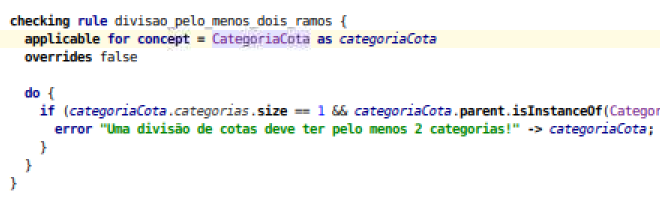
\includegraphics[width=0.85\textwidth]{chapters/dslcotas/mps/imagens/chekingrules.png}}

\par\medskip\textbf{Fonte:} Elaborada pelo autor (2020). \par\medskip

\end{figure}


\begin{figure}[ht!]
\centering

\caption{\textmd{Exemplo de \textit{quick fix}}}
\label{fig:quickfix}
\fcolorbox{gray}{white}{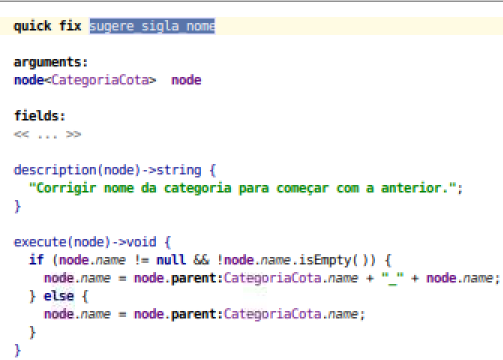
\includegraphics[width=0.85\textwidth]{chapters/dslcotas/mps/imagens/quickfixes.png}}

\par\medskip\textbf{Fonte:} Elaborada pelo autor (2020). \par\medskip

\end{figure}

\begin{figure}[ht!]
\centering

\caption{\textmd{Exemplo de \textit{inference rule}}}
\label{fig:inferencerule}
\fcolorbox{gray}{white}{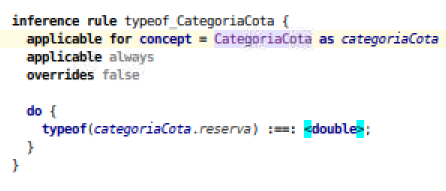
\includegraphics[width=0.85\textwidth]{chapters/dslcotas/mps/imagens/inferencerule.png}}

\par\medskip\textbf{Fonte:} Elaborada pelo autor (2020). \par\medskip

\end{figure}
